\chapter[Einleitung (Schmelzer)]{Einleitung}

%RGBD im Kommen
%Sensorik günstiger
%mobile Roboter

Mobile Roboter sind in den letzten Jahren immer weiter in den Fokus der Entwicklung gerückt. Sowohl im industriellen als auch im privaten Umfeld können sie ein breit gefächertes Spektrum von Aufgaben übernehmen. Weitere Einsatzgebiete sind in der Agrarwirtschaft, in Such- und Rettungsmissionen sowie im Katastrophenschutz und im Militär. Gerade in der Industrie können durch den Einsatz mobiler Roboter die Effizienz gesteigert und Arbeitsplätze gespart werden. Langfristig werden somit Kosten minimiert und die Sicherheit des Arbeitsumfelds verbessert. Außerdem eignen sich mobile Roboter besonders für den Einsatz in gefährlichem und unwegsamen Gelände, da Aufgaben, wie beispielsweise eine Bombenentschärfung, erledigt werden können ohne Menschen in Gefahr zu bringen.   

Mobile Roboter zeichnen sich dadurch aus, dass sie sich in ihrer Umgebung bewegen können und nicht, wie stationäre Roboter, an einen Ort gebunden sind. Die Abbildungen \ref{fig:stationär} bis \ref{fig:logistik} zeigen Beispiele verschiedener Roboter. In Abbildung \ref{fig:stationär} ist ein typischer stationärer Industrieroboter in Form eines Greifarms abgebildet. Auf den anderen Abbildungen sind verschiedene mobile Roboter dargestellt. Abbildung \ref{fig:staub} zeigt einen Staubsaugerroboter, Abbildung \ref{fig:feuer} einen Roboter für Einsätze im Katastrophenschutz und  Abbildung \ref{fig:logistik} einen Roboter von Boston Dynamics bei einer Logistik-Anwendung. 

\afterpage{
\begin{figure}[htb]
	\centering
	\begin{minipage}[t]{0.15\linewidth}
		\centering
		\includegraphics[width = \linewidth]{Bilder/stat_rob.png}
		\caption[Beispiel eines stationären Roboters in Form eines Greifarms]{Beispiel eines stationären Roboters in Form eines Greifarms\footnotemark}
		\label{fig:stationär}
	\end{minipage}
	\hfill
	\begin{minipage}[t]{0.2\linewidth}
		\centering
		\includegraphics[width = \linewidth]{Bilder/staubsaugerroboter.png}
		%\caption{Beispiel eines mobilen Staubsaugerroboters}
		\caption[Beispiel eines mobilen Staubsaugerroboters]{Beispiel eines mobilen Staubsaugerroboters\footnotemark}
		\label{fig:staub}
	\end{minipage}
	\hfill
	\begin{minipage}[t]{0.25\linewidth}
		\centering
		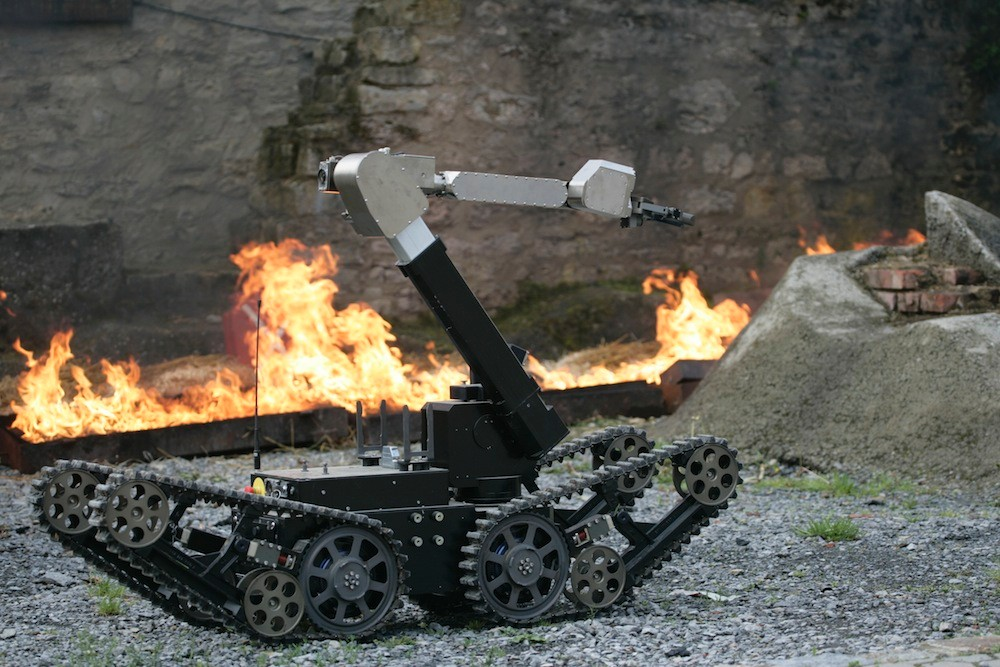
\includegraphics[width = \linewidth]{Bilder/feuerwehr.jpg}
		%\caption{Beispiel eines mobilen Roboters zum Einsatz im Katastrophenschutz}
		\caption[Beispiel eines mobilen Roboters zum Einsatz im Katastrophenschutz]{Beispiel eines mobilen Roboters zum Einsatz im Katastrophenschutz\footnotemark}
		\label{fig:feuer}
	\end{minipage}
	\hfill
	\begin{minipage}[t]{0.3\linewidth}
		\centering
		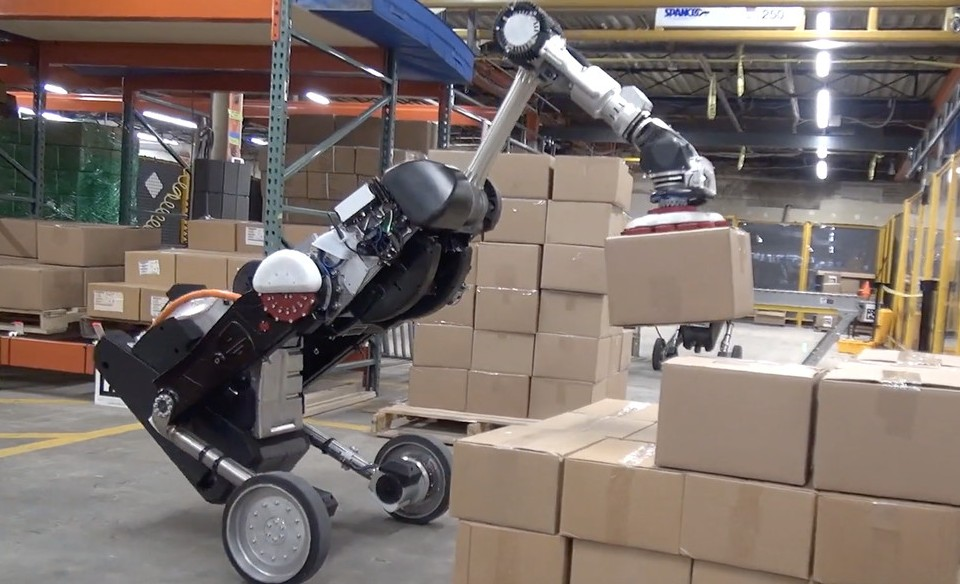
\includegraphics[width = \linewidth]{Bilder/industrie.jpg}
		%\caption{Beispiel eines mobilen Roboters bei einer Logistik-Anwendung}
		\caption[Beispiel eines mobilen Roboters bei einer Logistik-Anwendung]{Beispiel eines mobilen Roboters bei einer Logistik-Anwendung\footnotemark}
		\label{fig:logistik}
	\end{minipage}
\end{figure}
\addtocounter{footnote}{-3}
\footnotetext{\url{https://de.cleanpng.com/png-t0sbpe/}}
\stepcounter{footnote}
\footnotetext{\url{https://www.philips.de/c-m-ho/staubsauger/staubsauger-roboter/robotics}}
\stepcounter{footnote}
\footnotetext{\url{https://idw-online.de/de/news520138}}
\stepcounter{footnote}
\footnotetext{\url{https://www.technologyreview.com/s/613260/boston-dynamics-kinema-acquisition/}}
}

Da mobile Roboter nicht ortsgebunden sind, benötigen sie viel Sensorik und Rechenleistung, um ihre sich ständig ändernde Umgebung wahrzunehmen und verarbeiten zu können. Immer günstiger werdende Sensorik und Hardware sowie die steigende Leistungsfähigkeit bei gleichzeitig kleiner werdender Baugröße treiben die schnelle \linebreak Entwicklung mobiler Roboter voran. Außerdem ermöglichen Entwicklungen in anderen Forschungsgebieten, wie beispielsweise der künstlichen Intelligenz, neue Lösungsansätze für bestehende Probleme und erschließen neue Anwendungsfelder. 

Es gibt viele verschiedene Arten von mobilen Robotern. Sie unterscheiden sich anhand ihrer Konstruktion und Erscheinungsform, die sowohl an ihre Aufgaben als auch an die Umgebung, in der sie diese verrichten sollen, angepasst ist. Die Abbildungen \ref{fig:zipline} bis \ref{fig:cat} zeigen verschiedene mobile Roboter in unterschiedlichen Umgebungen. Sie können sowohl an Land, als auch in der Luft sowie auf und unter Wasser eingesetzt werden. Abbildung \ref{fig:zipline} zeigt eine Drohne, die in Afrika eingesetzt wird, um möglichst schnell Medikamente, Impfstoffe und Blutspenden an abgelegene Krankenhäuser auszuliefern. Auf Abbildung \ref{fig:spot} ist der Spot Mini von Boston Dynamics abgebildet, der auch Hindernisse überwinden kann. Das Institut für Systemdynamik der HTWG entwickelt mit dem Projekt CaRoLIME einen autonomen Wasserroboter, der autonom in unbekannten Umgebungen navigieren und arbeiten kann. Dieser ist auf Abbildung \ref{fig:cat} abgebildet. 

\afterpage{
\begin{figure}[htb]
	\centering
	\begin{minipage}[t]{0.3\linewidth}
		\centering
		\includegraphics[width = \linewidth]{Bilder/ghana.png}
		\caption[Ein unbemanntes Luftfahrzeug als Beispiel eines mobilen Roboters]{Ein unbemanntes Luftfahrzeug von Zipline zur Auslieferung von Medikamenten\footnotemark}
		\label{fig:zipline}
		%\footnotetext{\url{https://www.gemeinsam-fuer-afrika.de/ghana-medikamente-drohne/}}
	\end{minipage}
	\hfill
	\begin{minipage}[t]{0.3\linewidth}
		\centering
		\includegraphics[width = \linewidth]{Bilder/bostondynamics-spotmini.png}
		%\caption{Spot Mini von Boston Dynamics}
		\caption[Spot Mini von Boston Dynamics]{Spot Mini von Boston Dynamics\footnotemark}
		\label{fig:spot}
		%\footnotetext{\url{https://www.wevolver.com/wevolver.staff/spot.mini/}}
	\end{minipage}
	\hfill
	\begin{minipage}[t]{0.3\linewidth}
		\centering
		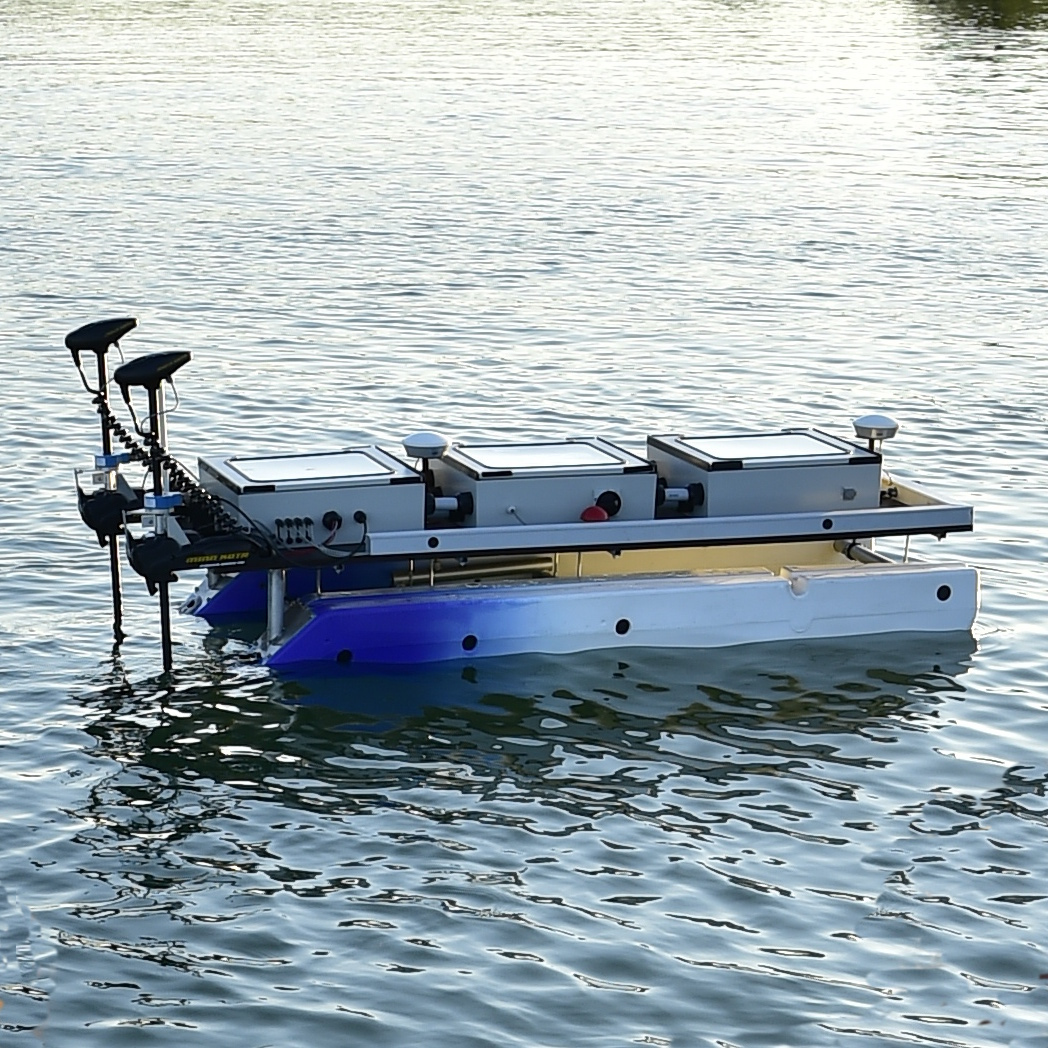
\includegraphics[width = \linewidth]{Bilder/CaRoLime.jpg}
		%\caption{Projekt CaRoLime des Instituts für Systemdynamik der HTWG}
		\caption[Projekt CaRoLime des Instituts für Systemdynamik der HTWG]{Projekt Ca\-Ro\-Lime des Instituts für Systemdynamik der HTWG\footnotemark}
		\label{fig:cat}
		%\footnotetext{\url{https://www.htwg-konstanz.de/forschung-und-transfer/institute-und-labore/isd/regelungstechnik/allgemein/}}
	\end{minipage}
\end{figure}
\addtocounter{footnote}{-2}
\footnotetext{\url{https://www.gemeinsam-fuer-afrika.de/ghana-medikamente-drohne/}}
\stepcounter{footnote}
\footnotetext{\url{https://www.wevolver.com/wevolver.staff/spot.mini/}}
\stepcounter{footnote}
\footnotetext{\url{https://www.htwg-konstanz.de/forschung-und-transfer/institute-und-labore/isd/regelungstechnik/allgemein/}}
}

%Die verschiedenen Konstruktionen und Erscheinungsformen sind sowohl an ihre Aufgaben als auch an die Umgebung, in der sie diese verrichten sollen, angepasst. 

Unabhängig von ihrem mit unter sehr verschiedenen Aufbau, Erscheinungsformen und Anforderungsprofil, haben alle mobilen Roboter gemeinsam, dass sie sich im Idealfall autonom auch in unbekannten Umgebungen zuverlässig orientieren müssen. Dafür müssen sie in der Lage sein eine genaue Karte der Umgebung zu erstellen sowie sich gleichzeitig in dieser zuverlässig zu lokalisieren. Dieses Verfahren wird %\ac{slam} 
Simultaneous Localization and Mapping (SLAM) genannt. 

\section[Motivation (Schmelzer)]{Motivation}

Bei SLAM-Verfahren basiert die Lokalisierung in der Karte auf dem Wiedererkennen schon einmal besuchter und kartierter Orte. Dies wird Place Recognition oder auch Loop Closure genannt. Hierfür gibt es verschiedene Ansätze, die sich in erster Li\-nie darin unterscheiden, wie der Roboter seine Umgebung wahrnimmt und verarbeitet. Häufig werden als Sensoren zur Umgebungswahrnehmung Kameras,LiDARs, Ultraschallsensoren oder Radars eingesetzt. 

Bildbasierte SLAM-Verfahren leiden häufig unter Fehleranfälligkeit bei Beleuchtungs- oder Blickwinkeländerungen. LiDAR-Sensoren liefern Entfernungsmessungen in Form von Punktwolken mit Hilfe derer die Umgebung in hoher Auflösung anhand ihrer Strukturen wahrgenommen wird. Daher wird die Qualität LiDAR-basierter SLAM-Verfahren nicht durch Beleuchtungsänderungen beeinflusst. Außerdem sind die Auswirkungen von Blickwinkeländerungen geringer.  

Um Loop Closures erfolgreich erkennen zu können, müssen  verschiedenen Orte eindeutig unterscheidbar beschrieben werden. Hierfür gibt es verschiedene Ansätze. Ein häufig verwendeter Ansatz ist das Wiedererkennen markanter Punkte in den Punkt\-wol\-ken, sogenannte Keypoints. Diese sind jedoch nicht immer eindeutig unterscheidbar und die Wiedererkennung ist abhängig vom Blickwinkel. Ein weiterer Ansatz ist das Matchen von Objekten, die aus den Punktwolken extrahiert werden. Diese Art der Umgebungswahrnehmung ist ähnlicher zur menschlichen Wahrnehmung. Außerdem können Karten auf Basis von Objekten besser Situationen repräsentieren, in denen statische Objekte dynamisch werden. 

Ein Nachteil bei der Repräsentation der Umgebung anhand von Objekten ist, dass sich reale Umgebungen häufig nicht ausschließlich aus tatsächlichen Objekten, die eindeutig unterscheidbar sind, zusammensetzen. Außerdem wird ein perfekter Objektsegmentierungsalgorithmus benötigt. 

Einen anderen Ansatz verwendet der SegMap-Algorithmus. Dieser wurde am Autonomous Systems Lab der ETH Zürich entwickelt. Die Umgebung wird mit Hilfe eines LiDAR-Sensors in Form einer dreidimensionalen Punkt\-wol\-ke wahrgenommen. Die Struktur und der Aufbau der Umgebung wird durch Segmente repräsentiert, die aus der Punkt\-wol\-ke extrahiert werden. Dies müssen nicht unbedingt abgeschlossene Objekte sein, sondern können auch nur Teile von Objekten oder Teile größerer Strukturen, wie Fenster oder Türen in Häuserfassaden, sein. Dadurch werden die Pro\-bleme, die Objekt-basierte SLAM-Verfahren haben, umgangen. Außerdem wird keine umfassende Datenbank benötigt, die die diversen Objektklassen enthält. Abbildung \ref{fig:segmente} zeigt Beispiele von Segmenten. Zu sehen sind ein Teil einer Häuserfassade, ein Baum sowie ein Fahrzeug.

\begin{figure}
    \centering
    \includegraphics[width=\linewidth]{Bilder/segmente.png}
    \caption[Beispiele für Segmente]{Beispiele für Segmente \cite{Dube2017a}}
    \label{fig:segmente}
\end{figure}

Das Verfahren ist für urbane outdoor-Anwendungen konzipiert. Tests haben gezeigt, dass gute Ergebnisse erreicht werden und eine zuverlässige Lokalisierung möglich ist.

Da dreidimensionale LiDAR-Sensoren sehr teuer sind, ist das Verfahren ungeeignet zur Anwendung auf kleinen und günstigen mobilen Robotern, die oft für indoor-Anwendungen verwendet werden. Zuverlässige SLAM-Verfahren sind jedoch gerade in indoor-Umgebungen wichtig, da globale  Positionsinformationen, wie z.B. GPS-Daten, fehlen und nur mit hohem Aufwand zur Verfügung gestellt werden können, wie beispielsweise über Beacons oder externe Tracking-Kameras. Außerdem bietet die hohe Reichweite von LiDAR-Sensoren für indoor Anwendungen in den meisten Fällen keinen Mehrwert. 

Für kompakte, leichte und günstige mobile Roboter zur Anwendung in indoor-Um\-ge\-bung\-en, deren Orientierung auf Basis von Strukturen arbeitet, bieten sich RGB-D Kameras an. Diese liefern neben einem Farbbild ähnlich wie LiDAR-Sensoren ebenfalls Tiefeninformationen in Form von Punktwolken. 

\section[Ziel der Arbeit (Schmelzer)]{Ziel der Arbeit}

Das Ziel dieser Arbeit ist die Anwendung des SegMap-Algorithmus auf indoor-Um\-ge\-bung\-en mit den Daten einer RGB-D Kamera. Hierfür werden die Werte diverser Parameter experimentell ermittelt. Außerdem werden eventuell nötige Änderungen am Algorithmus vorgenommen, die die Lokalisierungsergebnisse verbessern sollen. Die Anwendung des Algorithmus auf RGB-D Daten in indoor-Szenarien wird anhand verschiedener Datensätze validiert. 

%Das Ziel dieser Arbeit ist die Anwendung des SegMap-Algorithmus auf indoor-Um\-ge\-bung\-en mit den Daten einer RGB-D Kamera. Hierfür werden die Werte diverser Parameter experimentell ermittelt und eventuell nötige Änderungen am Algorithmus vorgenommen. Da die Reichweite einer RGB-D Kamera wesentlich geringer ist als die eines LiDAR-Sensors, wird die Anwendung des Algorithmus auf RGB-D Daten in indoor-Szenarien ausgewertet. 

%. Eine RGB-D Kamera bietet im Gegensatz zu LiDAR-Sensoren zusätzlich den Vorteil, dass sie neben den Tiefeninformationen auch Farbinformationen liefert. Daher werden die im Algorithmus verwendeten Segmentierungsmethoden um eine Berücksichtigung der Farbwerte erweitert. 

%eventuell nötige Anpassungen am Code vorgenommen. Da die Reichweite einer RGB-D Kamera wesentlich geringer ist als die eines LiDAR-Sensors, wird die Anwendung des Algorithmus auf RGB-D Daten in indoor-Szenarien ausgewertet. 

%Eine RGB-D Kamera bietet zusätzlich den Vorteil, dass sie neben den Tiefeninformationen gleichzeitig auch RGB-Bilder liefert. Daher wird ein Ansatz ausgearbeitet den SegMap-Algorithmus durch ein visuelles SLAM-verfahren zu erweitert. Ob durch die Fusionierung eine Verbesserung des SegMap-Algorithmus erzielt wird, wird ebenfalls verifiziert. 

\section[Gliederung und Aufbau (Schmelzer)]{Gliederung und Aufbau}

Die Arbeit ist so aufgeteilt, dass in den Kapiteln 2 bis 4 zunächst Grundlagen erklärt werden, die für das Verständnis der Arbeit wichtig sind. Anschließend wird in Kapitel 5 die Funktionsweise des SegMap-Algorithmus erklärt sowie die Änderungen an diesem präsentiert. In den Kapiteln 6-8 wird erläutert, wie das SegMap-Verfahren auf die Anwendung von RGB-D Daten in indoor-Umgebungen übertragen wird. Abschließend werden in Kapitel 9 die Ergebnisse evaluiert sowie ein Fazit über die Arbeit gezogen. Außerdem wird ein kurzer Ausblick über sinnvolle weitere Änderungen und Erweiterungen des Algorithmus gegeben, um die Anwendbarkeit auf indoor-Umgebungen mit RGB-D Daten weiter zu verbessern.


%Außerdem wird der Fusionierungsansatz erklärt sowie die Evaluierung präsentiert. Abschließend wird ein Fazit der Arbeit gezogen und ein kurzer Ausblick über sinnvolle Erweiterungen und weitere Experimente gegeben. 
